%%%%%%%%%%%%%%%%%%%%%%%%%%%%%%%%%%%%%%%%%%%%%%%%%%%%%%%%%%%%%%%%%%%%%%%%%%%%%%%%
%2345678901234567890123456789012345678901234567890123456789012345678901234567890
%        1         2         3         4         5         6         7         8

\documentclass[letterpaper, 10 pt, conference]{ieeeconf}  % Comment this line out
                                                          % if you need a4paper
%\documentclass[a4paper, 10pt, conference]{ieeeconf}      % Use this line for a4
                                                          % paper

\IEEEoverridecommandlockouts                              % This command is only
                                                          % needed if you want to
                                                          % use the \thanks command
\overrideIEEEmargins
% See the \addtolength command later in the file to balance the column lengths
% on the last page of the document
\usepackage{subcaption}
\usepackage{graphicx}
\usepackage{listings}
\graphicspath{{./graph/}}

% The following packages can be found on http:\\www.ctan.org
%\usepackage{graphics} % for pdf, bitmapped graphics files
%\usepackage{epsfig} % for postscript graphics files
%\usepackage{mathptmx} % assumes new font selection scheme installed
%\usepackage{times} % assumes new font selection scheme installed
%\usepackage{amsmath} % assumes amsmath package installed
%\usepackage{amssymb}  % assumes amsmath package installed

\title{\LARGE \bf
ROS2 for Robot Mapping and Navigation
}

\author{Zoe Li \\
        Zoe.Li@bshg.com% <-this % stops a space
}
\begin{document}

\maketitle
\thispagestyle{empty}
\pagestyle{empty}
%%%%%%%%%%%%%%%%%%%%%%%%%%%%%%%%%%%%%%%%%%%%%%%%%%%%%%%%%%%%%%%%%%%%%%%%%%%%%%%%
\begin{abstract}
 This guide gives an overview of ROS2 status with an example of SLAM implementation. ROS2 is an upgrade after one decade since the introduction of ROS (Robotic Operating System) and is still under heavy development at this moment as June 2019. In this guide, we discuss and evaluate some of its new features by implementing SLAM in ROS2 in simulation and on a real robot. These new features are briefly introduced and some are tested in this implementation. A demo with source code is provided in the end of the paper.
\end{abstract}
%%%%%%%%%%%%%%%%%%%%%%%%%%%%%%%%%%%%%%%%%%%%%%%%%%%%%%%%%%%%%%%%%%%%%%%%%%%%%%%%
\section{INTRODUCTION}
\subsection{Robot Operating System Background}
Robot Operating System (ROS) is a robotics middleware that was created by Willow Garage and Stanford University and now maintained by Open Source Robotics Foundation(OSRF)\cite{c2}.  As an open source framework for various robotics software development, ROS provides functions such as hardware abstraction, device control, message passing, package management and libraries for different functionalities. The modulated packages of ROS allows users to focus on application development rather than spending much effort to reinvent the wheel.
%%%%%%%%%%%%%%%%%%%%%%%%%%%%%%%%%%%%%%%%%%%%%%%%%%%%%%%%%%%%%%%%%%%%%%%%%%%%%%%%
\subsection{ROS2 Design Background}
ROS was originally designed for PR2 use case. PR2 robot works as a standalone robot with excellent network connectivity, also PR2 applications are mostly research based, therefore the early design concept of ROS does not need to consider real-time problems.

Nowadays ROS has gained tremendous popularity in robotics community, and the use cases has grown beyond the scope of academia and scientific research. Many robotics applications such as  industrial robots, outdoor robots(for example driver-less cars), unmanned aerial vehicles(UVA) have become more and more complicated, as a result, those applications have higher demand on the robust real-time performance of the robot operating system. Although ROS1 is still a very popular development tool in the field of robotics, the limitations of the original design have become a driving force of the new ROS2 design\cite{c3}. 

With the growing demand of cross operating system platform and real-time functionality from the ROS community, ROS2 development was first announced at ROSCon 2014, and the first alpha version was launched in August 2015. On December 8, 2017, the highly anticipated ROS 2.0 finally released its first official version, Ardent Apalone. As of 2019, the newest version ROS 2 Dashing Diademata was released on May 30.

Compare to ROS1, ROS2 has the following support for robotics applications\cite{c3}: 
\begin{itemize}
  \item \textbf{Cross-system platform support}: ROS2 support for Linux, Windows and macOS as well as the real-time operating system(RTOS).
  \item \textbf{Multi-robot system support}: Improved communication system allows robust network performance for multi-robot system 
  \item \textbf{Real-time control}: support to improve the timeliness of a robot control application and overall robot performance
  \item \textbf{Non-ideal networks}: Support robot appications such as UAV, underground robot or underwater robot that has bad networks connection compare to indoor robots 
  \item \textbf{Production environments}: ROS 1 has target users as research labs, while ROS 2 is suitable for real-world applications. 
  \item \textbf{Small embedded platforms}:ROS 2 does not rely on a master to distribute messages, and its native UDP communication system performs much better on distributed embedded system\cite{c6}. 
\end{itemize}

\subsection{ROS2 Communication}
\begin{figure}[ht]
  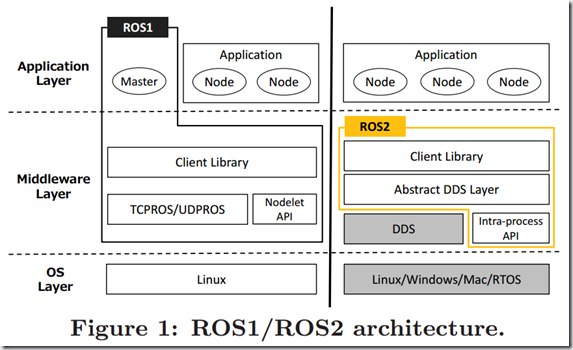
\includegraphics[width=\linewidth]{ros1_ros2_architecture.png}
  \caption{ROS1/ROS2 Architecture \cite{c1}} 
  \label{fig:ros2_architecture}
\end{figure}

ROS1 uses TCP (Transmission Control Protocol) as its communication protocol. TCP is a connection oriented network, this means that TCP tracks all data sent, requiring acknowledgment for each octet (generally), therefore,  ROS1 has a centralized network configuration which requires a running ROS master to take care of naming and registration services. With the help of the master, ROS nodes could find each other on the network and communicate in a peer-to-peer fashion. In ROS1 setting, all nodes will depend on the central ROS master. When the network becomes lossy and unstable(especially if nodes are distributed on several computers), the communication will not be reliable for real-time applications or multi-robot systems.

ROS2 uses Data Distribution Service (DDS) as the communication middleware. UDP is a Data-Centric-Publish-Subscribe(DCPS) model, and this model will create global data space for individual applications to exchange information. DDS will identify a data object by its topic name and then subscribe to this topic, therefore, DDS does not have a central distributor for all information. The DDS publish-subscribe model avoids complex network programming for distributed applications.  ROS2 provides an abstraction layer of DDS, so users do not need to pay attention to the underlying DDS structure. The ROS2 Middleware Interface(RMW) allows users to choose different Quality of Service(QoS). The real-time publish-subscribe (RTPS) protocol allows ROS2 nodes to automatically find each other on the network, thus there is no need for a ROS2 master. This is an important point in terms of fault tolerance.


\subsection{ROS 2 QoS policy}

%%%%%%%%%%%%%%%%%%%%%%%%%%%%%%%%%%%%%%%%%%%%%%%%%%%%%%%%%%%%%%%%%%%%%%%%%%%%%%%%
\section{Related Work}
When ROS 2 Bouncy was released, a TurtleBot 2 demo was provided to demonstrate the some popular mapping and localization packages that runs in ROS 2. TurtleBot 2 demo uses Google Cartographer to get maps of the environment, and use AMCL (Adaptive Monte Carlo Localization)package to localize. TurtleBot 2 demo also provided TurtleBot 2 driver and the Orbbec Astra depth camera sensor driver. At the time this demo was created, ROS 2 navigation stack was still under development, therefore, TurtleBot 2 demo uses joystick to manually operate the robot to create maps. 

After ROS 2 Dashing was released, The manufacturer of TurtleBot 3 ROBOTIS\cite{c5} provided a TurtleBot 3 demo that runs ROS 2 dashing. TurtleBot 3 demo includes robot mapping and navigation, so this demo for Kobuki robot is based on the work of TurtleBot 3. 
%%%%%%%%%%%%%%%%%%%%%%%%%%%%%%%%%%%%%%%%%%%%%%%%%%%%%%%%%%%%%%%%%%%%%%%%%%%%%%%%
\section{Method}
The objective of this demo is to build a Kobuki SLAM and navigation demo on top of the existing TurtleBot 2 demo, and update packages so that the Kobuki robot can achieve SLAM and autonomous navigation using the latest ROS 2 Dashing Diademata release. 
 
\begin{figure}[ht]
  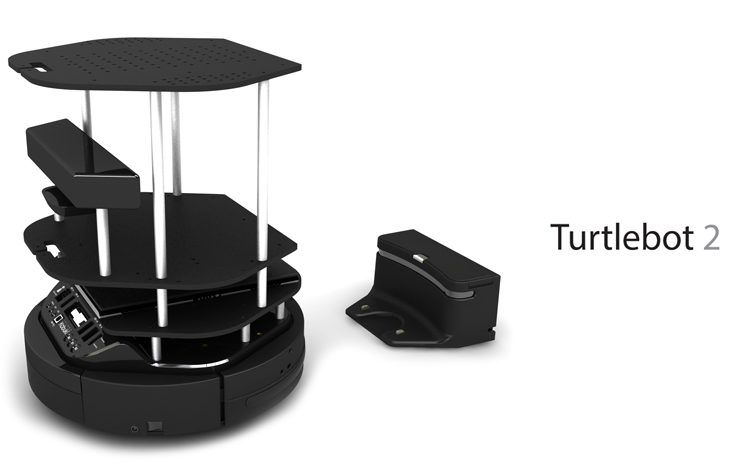
\includegraphics[width=\linewidth]{kobuki_image.jpg}
  \caption{Image of Kobuki Robot(TODO)} 
  \label{fig:Kobuki_image}
\end{figure}
%%%%%%%%%%%%%
\subsection{Hardware and software setup}
\begin{itemize}
\item  Hardware setup 
    \begin{itemize}
        \item Robot: Kobuki (turtlebot2)
        \item Sensor: hokuyo laser scanner
    \end{itemize}{}
\end{itemize}

\begin{itemize}
\item ROS2 Packages:
    \begin{itemize}
        \item Mapping   
            \begin{itemize}
                \item cartographer (binary release available)
                \item cartographer-ros 
            \end{itemize}{}
    \end{itemize}{}
    \begin{itemize}
        \item Navigation
            \begin{itemize}
                \item Navigation2 
            \end{itemize}{}
    \end{itemize}{}
    \begin{itemize}
        \item Visualization
            \begin{itemize}
                \item ros1\_bridge (binary release available)
                \item rviz
            \end{itemize}{}
   
        \item Controller and drivers:
            \begin{itemize}
                \item teleop\_twist\_keyboard (binary release available)
                \item urg\_node: URG laser scan driver 
                \item tutlebot2\_drivers: provide kobuki\_node to drive the Kobuki Robot
            \end{itemize}{}
        \item Simulation:
            \begin{itemize}
                \item Gazebo9 simulation (binary release available)
            \end{itemize}{}
    \end{itemize}{} 
\end{itemize}{}

\begin{itemize}
    \item Simulation 
        \begin{itemize}
            \item Gazebo simulation environment 
            \item Kobuki model 
            \item Gazebo differential drive plug-in  
            \item Gazebo sensor plug-in 
        \end{itemize}{}
\end{itemize}{}

%%%%%%%%%%%%%
\subsection{Implementation}

% 1. Change CmakeList.txt and package.xml
% 2. Build all packages using colcon build 
% 3. Manually control robot and use Goolge Cartographer to get the map 
% 4. Visualization using ros1_bridge 
1. \textit{Setup Build files} \par \vspace{5pt}
 ROS2 uses a build system called Ament Build tool. Ament is an evolution of catkin that automatically build a set of independent packages base on their dependency topological order. Ament will also install and configure the environment for packages, so the user does not need to follow a specific dependency order to build packages. The package.xml will provide meta information about the packages and their dependencies, and the build configuration are stored in the CMakeList.txt  \par \vspace{5pt}
 
2. \textit{Build packages using colcon build}\par\vspace{5pt}
ROS1 has multiple different building tools such as catkin\_make, catkin\_make\_isolated and catkin\_tools. ROS 2 provides a universal build tool called colcon. This colcon tool makes the building testing and using multiple packages easy\cite{c7}. \par\vspace{5pt}

3. \textit{Manual mapping using Cartographer}\par\vspace{5pt} TODO Kobuki\_driver SetUp \par\vspace{5pt}
% launch system 
This demo uses teleop-keyboard to manually operate the Kobuki robot. The cartographer node utilizes the laser scan data obtained from the hokuyo laser scanner and the optometry information published though the kobuki\_node robot driver and create a 2D map. 
This demo uses teleo-keyboard to operate the Kobuki robot, and obtain a map using google cartographer. The rqt\_graph of the structure is show in figure \ref{fig:rqt}\par\vspace{5pt}
\begin{figure}[ht]
  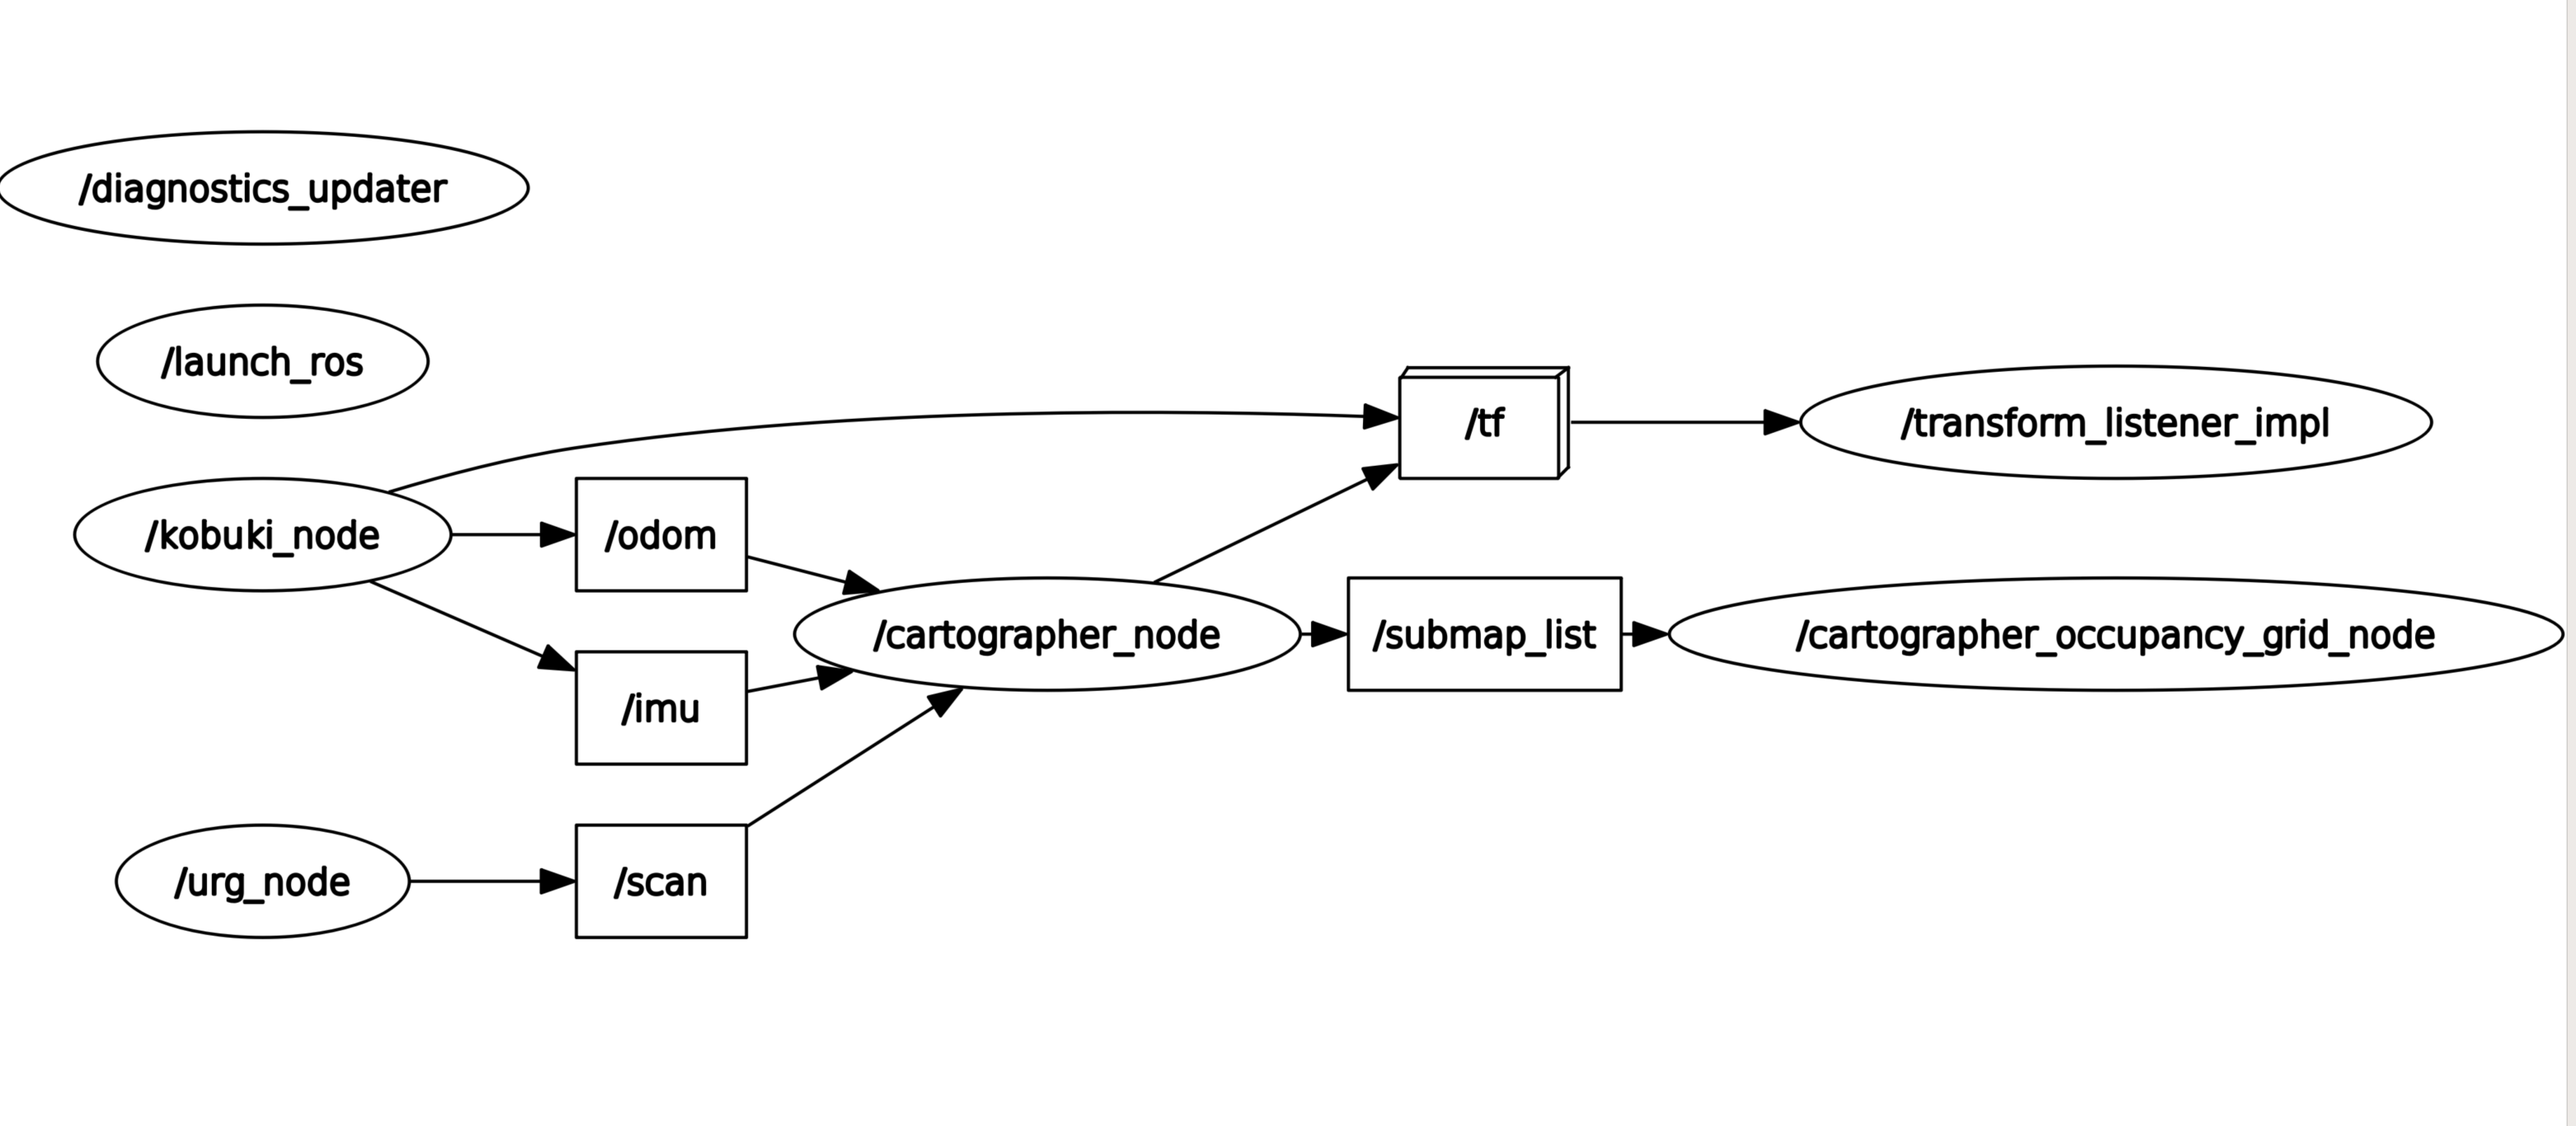
\includegraphics[width=\linewidth]{qrt_graph.png}
  \caption{ROS2 rqt\_graph} 
  \label{fig:rqt}
\end{figure}
4. \textit{Data visualization using ros1\_bridge}\par\vspace{5pt} 
ROS 2 is still under heavy development, so many packages built for ROS 1 have not yet been converted into ROS 2 compatible version. ROS 2 designers provided a solution to bridge the communication between ROS 1 and ROS 2 by ros1\_bridge.  

This demo uses ros1\_bridge to pass data into ROS 1 to visualize the map obtained by cartographer. ros1\_bridge provides a network bridge which enables the exchange of messages between ROS 1 and ROS 2. This bridge will establish connection when matching publisher-subscriber pairs are active to a topic on either side of the bridge\cite{c4}. The current version supports most of the common message types in ROS 1 and ROS 2, user can also create their own customized message pairs through a package mapping rule file that matches all messages with the same names and fields within a pair of packages.\par\vspace{5pt} 

5. \textit{Launch File Setup} \par\vspace{5pt}
ROS 2 launch system are very different compare to ROS 1, it uses python script to launch applications and describe configurations. Python launch file has very little prescribed structure, which gives uses lots of flexibility. For example, this demo uses python OS (operating system interfaces) to directly set the gazebo model path environment variable, so users do no have to manually enter this environment variable into the terminal shell. 
\par\vspace{2pt}
\begin{small}
\begin{verbatim}
os.environ['GAZEBO_MODEL_PATH'] =
gazebo_model_path
\end{verbatim}
\end{small}
\par\vspace{2pt}
Also ROS 2 has a new system of setting parameters in launch files. ROS 2 stores parameters of a node in a \textit{.yaml} file and pass the \textit{.yaml} file as a launch argument. The following code shows a example of launching urg\_node in this demo: \par\vspace{2pt}
\begin{small}
\begin{verbatim}
launch_ros.actions.Node(
    package="urg_node",
    node_executable="urg_node",
    output="screen",
    arguments=["__params:=/PATH/urg.yaml"])
\end{verbatim}
\end{small}\par\vspace{2pt}
The following is an example of urg\_node parameter file in ROS 2 setting: 
\begin{small}
\begin{verbatim}
urg_node:
  ros__parameters:
    angle_max: 3.14
    angle_min: -3.14
    ip_port: 10940
    serial_port: "/dev/ttyACM0"
    serial_baud: 115200
    laser_frame_id: "laser"
    calibrate_time: false
    default_user_latency: 0.0
    diagnostics_tolerance: 0.05
    diagnostics_window_time: 5.0
    error_limit: 4
    get_detailed_status: false
    publish_intensity: false
    publish_multiecho: false
    cluster: 1
    skip: 0
\end{verbatim}
\end{small}{}
6. \textit{Simulation Setup} \par\vspace{5pt} 
In this demo, simulation environment was modeled as the Bosch Sunnyvale office. The simulated office settings shown in figure\ref{fig:gazebo} has walls and desks as obstacles for the robot to perform mapping and navigation. \begin{figure}[ht]
  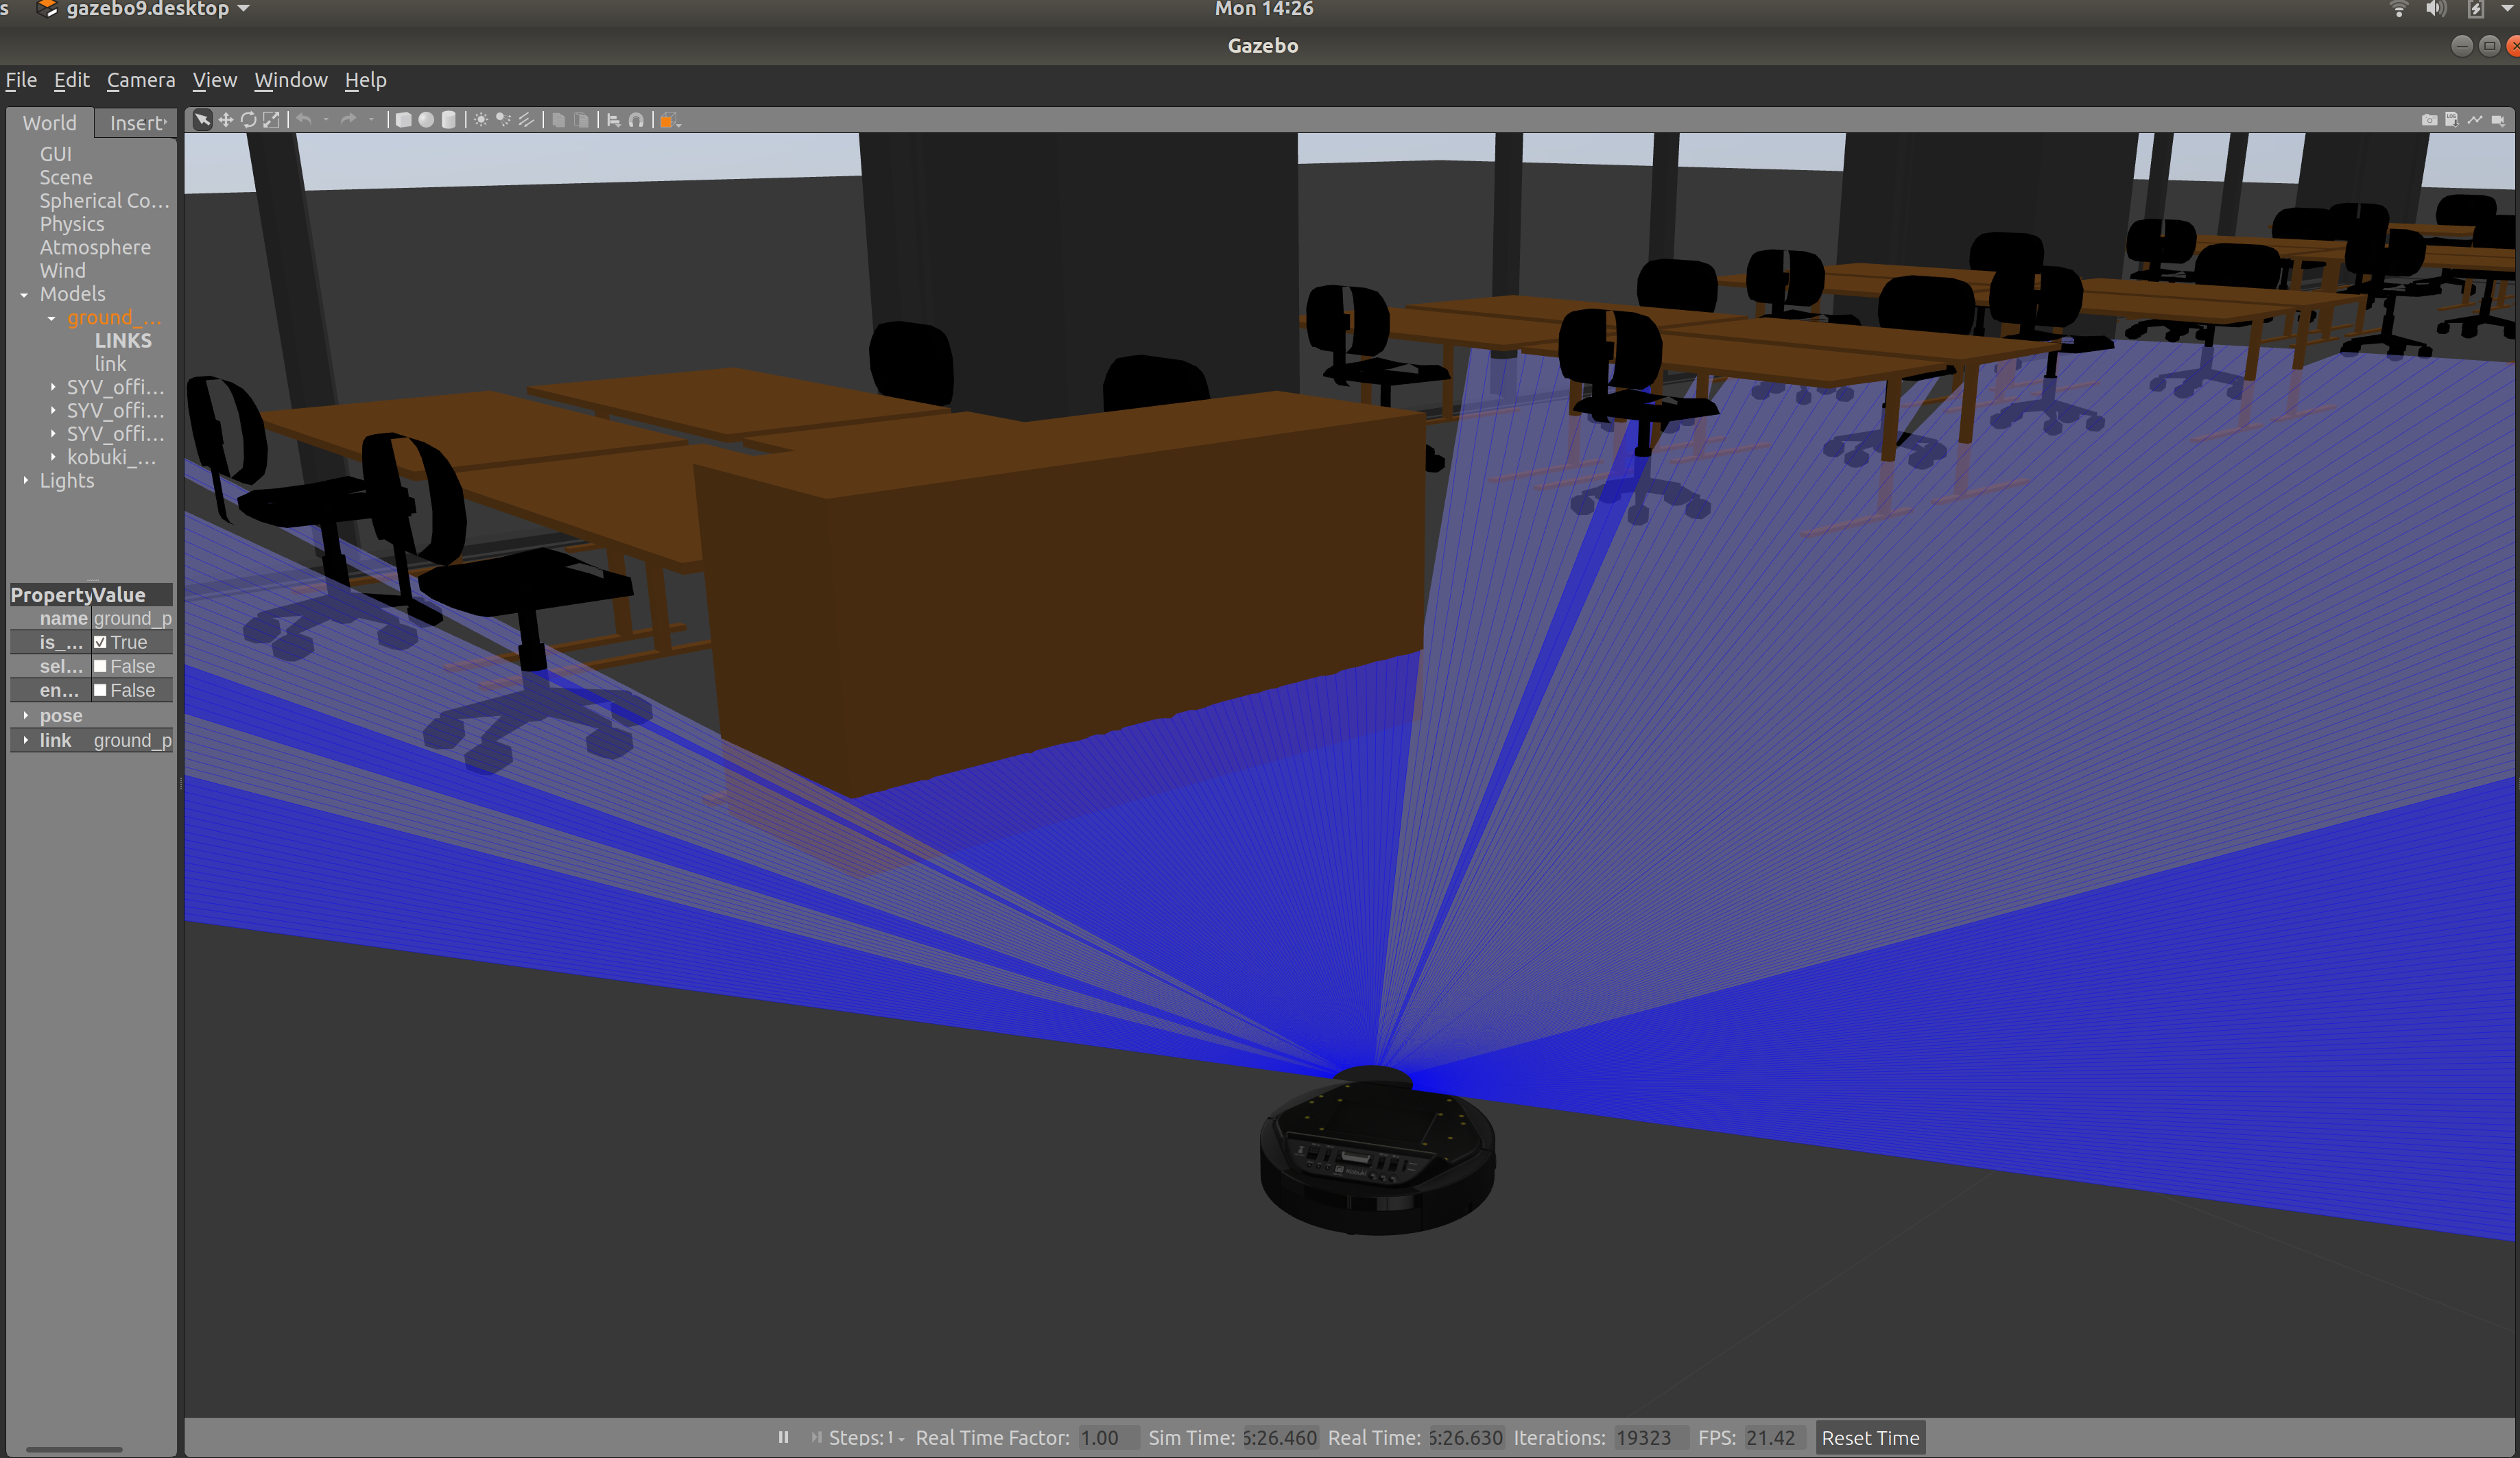
\includegraphics[width=\linewidth]{gazebo_simulation.png}
  \caption{Kobuki and laser scanner in Gazebo 9 Simulation } 
  \label{fig:gazebo}
\end{figure}
\par\vspace{5pt} 

7. \textit{Navigation in simulation} \par\vspace{5pt} 
The navigation 2 package is designed for ROS 2, just like the original navigation stack in ROS 1, navigation 2 enables a robot to autonomously reach a goal state. Kobuki navigation uses the navigation2 packages to navigate through the map obtained by google cartographer. Given a robot initial pose, and a goal pose shown in rviz map, navigation 2 will generate a path plan and send command to the drive the robot. The robot will reach the goal while avoiding obstacles along the path. 
%%%%%%%%%%%%%%%%%%%%%%%%%%%%%%%%%%%%%%%%%%%%%%%%%%%%%%%%%%%%%%%%%%%%%%%%%%%%%%%%
\section{Results}\label{results}
\subsection{Robot Mapping}
The map shown in figure \ref{fig:map} was obtained by driving the robot in a room. The result draws reasonable boundaries. However area that near large windows shows a large amount of noise due to laser reflection. 
\begin{figure}[ht]
  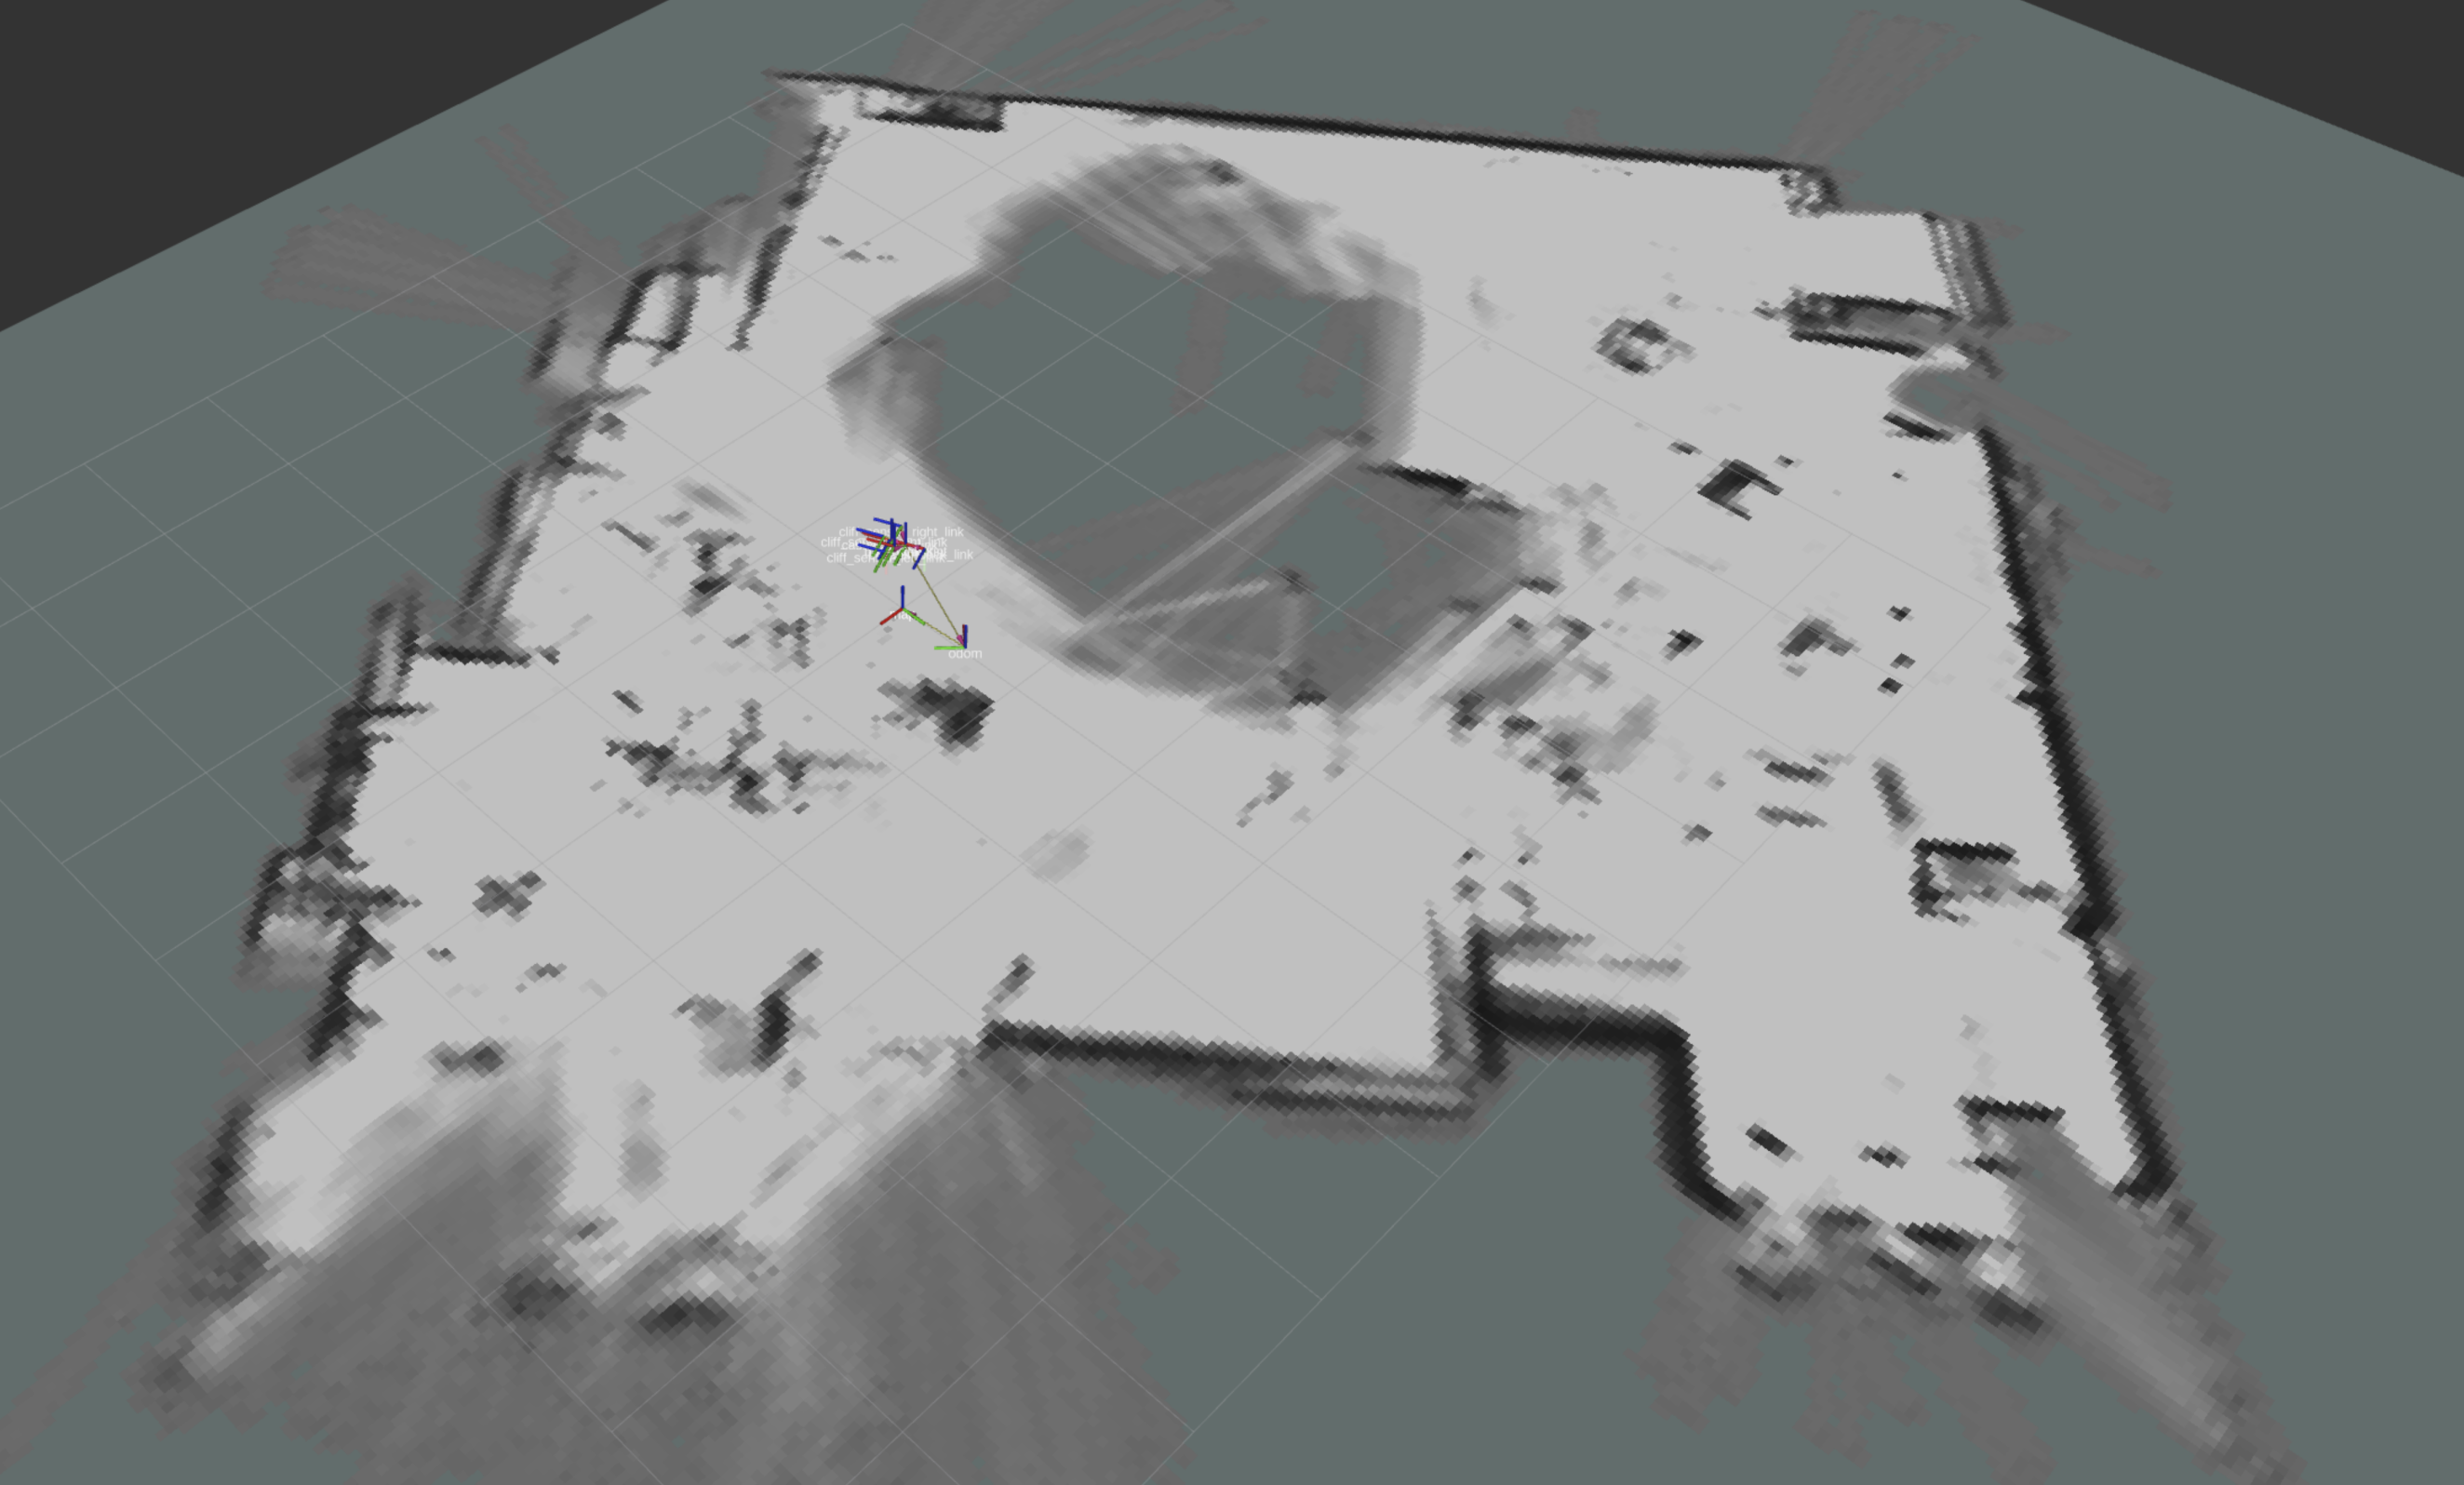
\includegraphics[width=\linewidth]{map.png}
  \caption{map obtained by google cartographer} 
  \label{fig:map}
\end{figure}
\subsection{Gazebo 9 Simulation}
The AMCL localization and navigation works well in simulation. However, due to lack of landmarks, the localization result is highly depend on how the use select the initial position.
    \begin{figure}[ht]
    \begin{subfigure}[b]{0.5\textwidth}
       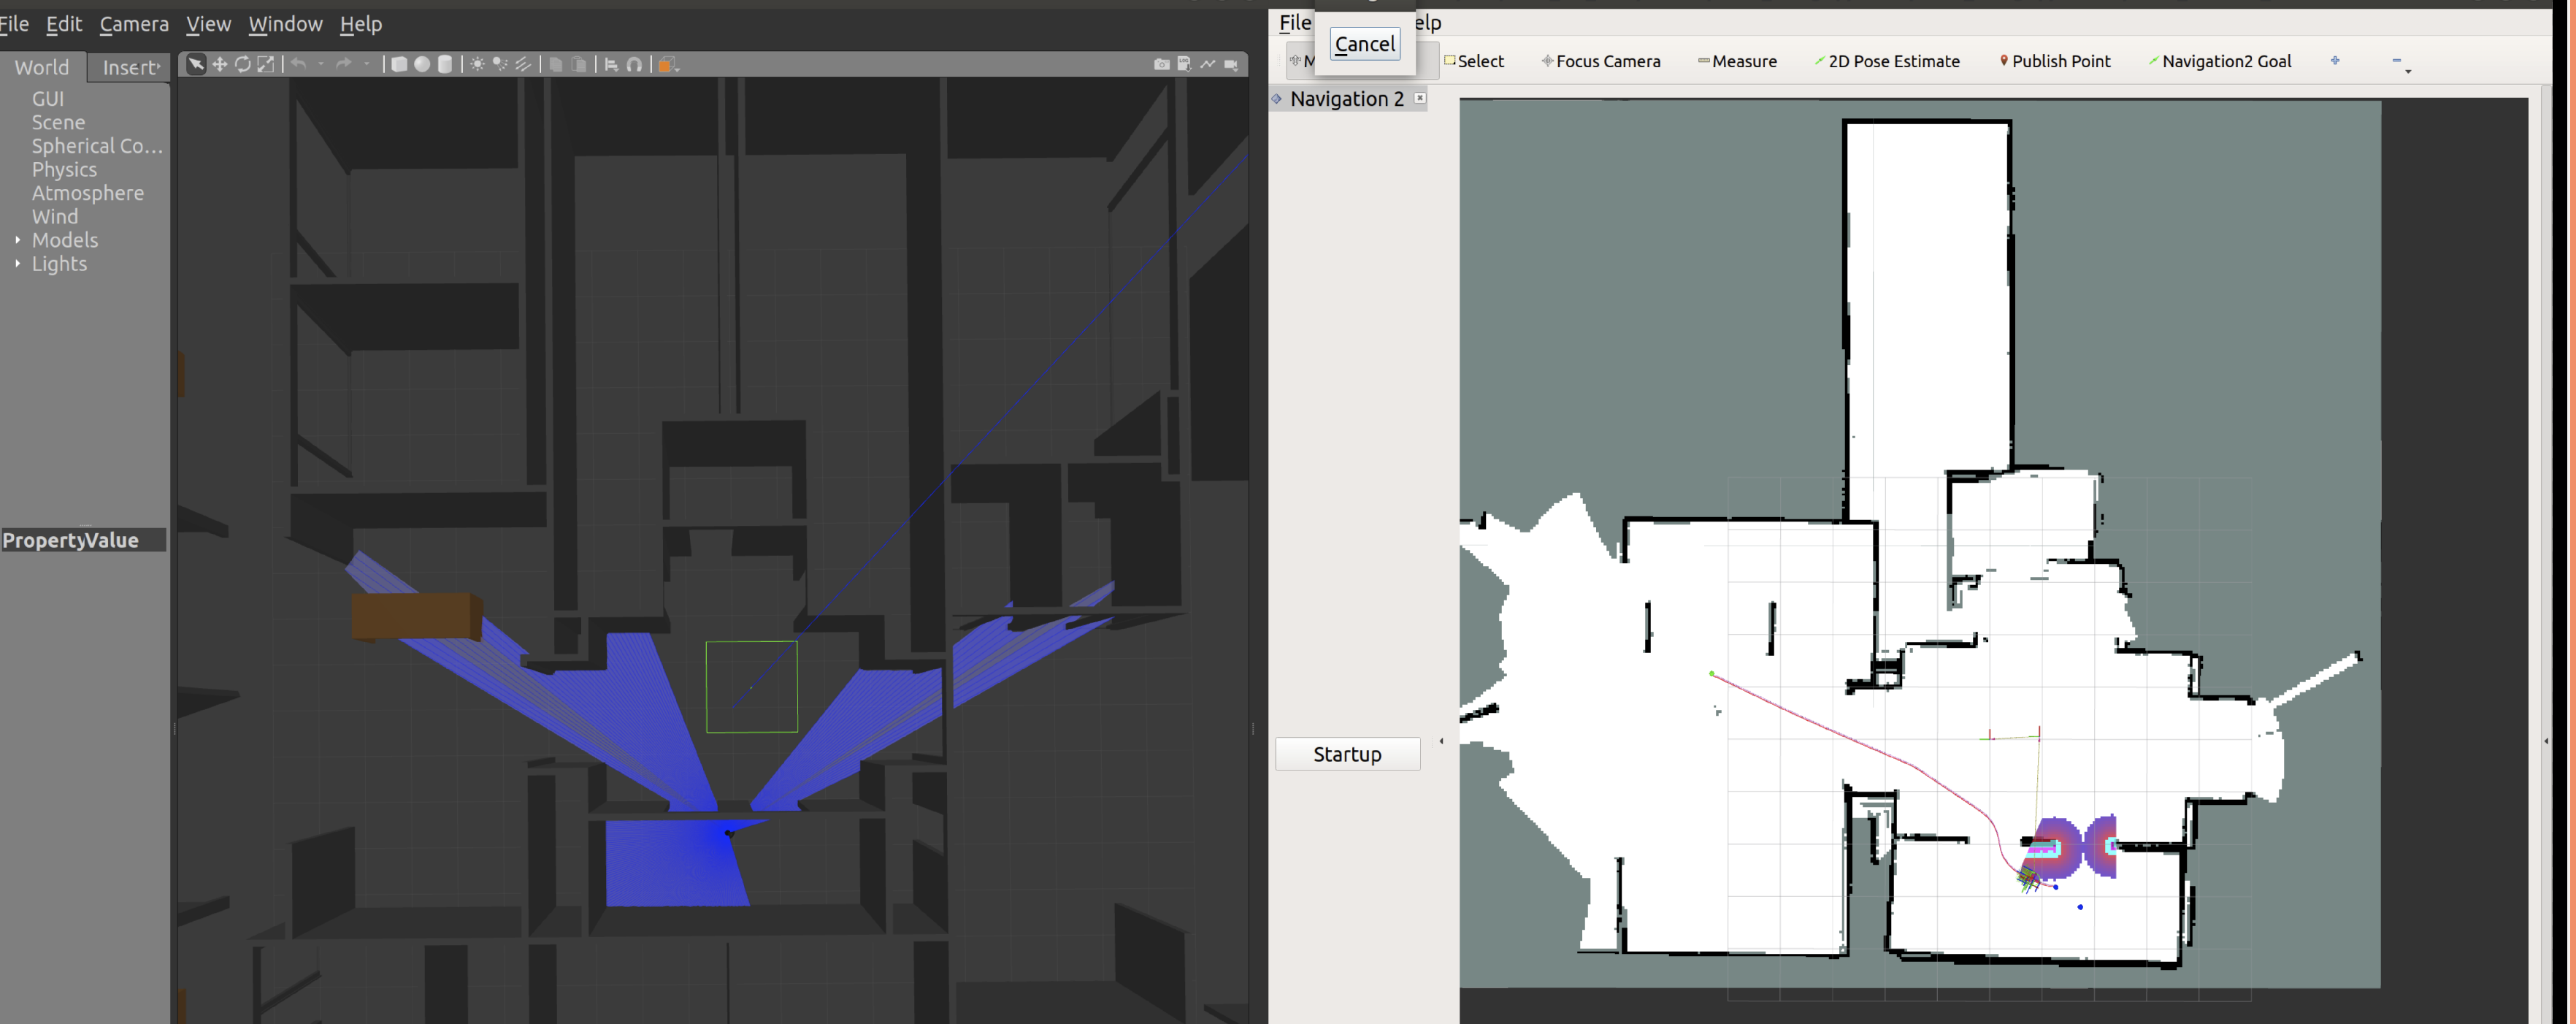
\includegraphics[width=1\linewidth]{navigation.png}
       \caption{Starting point of navigation}
       \label{fig:Ng1} 
    \end{subfigure}
    
    \begin{subfigure}[b]{0.5\textwidth}
       \includegraphics[width=1\linewidth]{navigation2.png}
       \caption{Midpoint of the navigation}
       \label{fig:Ng2}
    \end{subfigure}
\end{figure}

\begin{figure}[ht]
  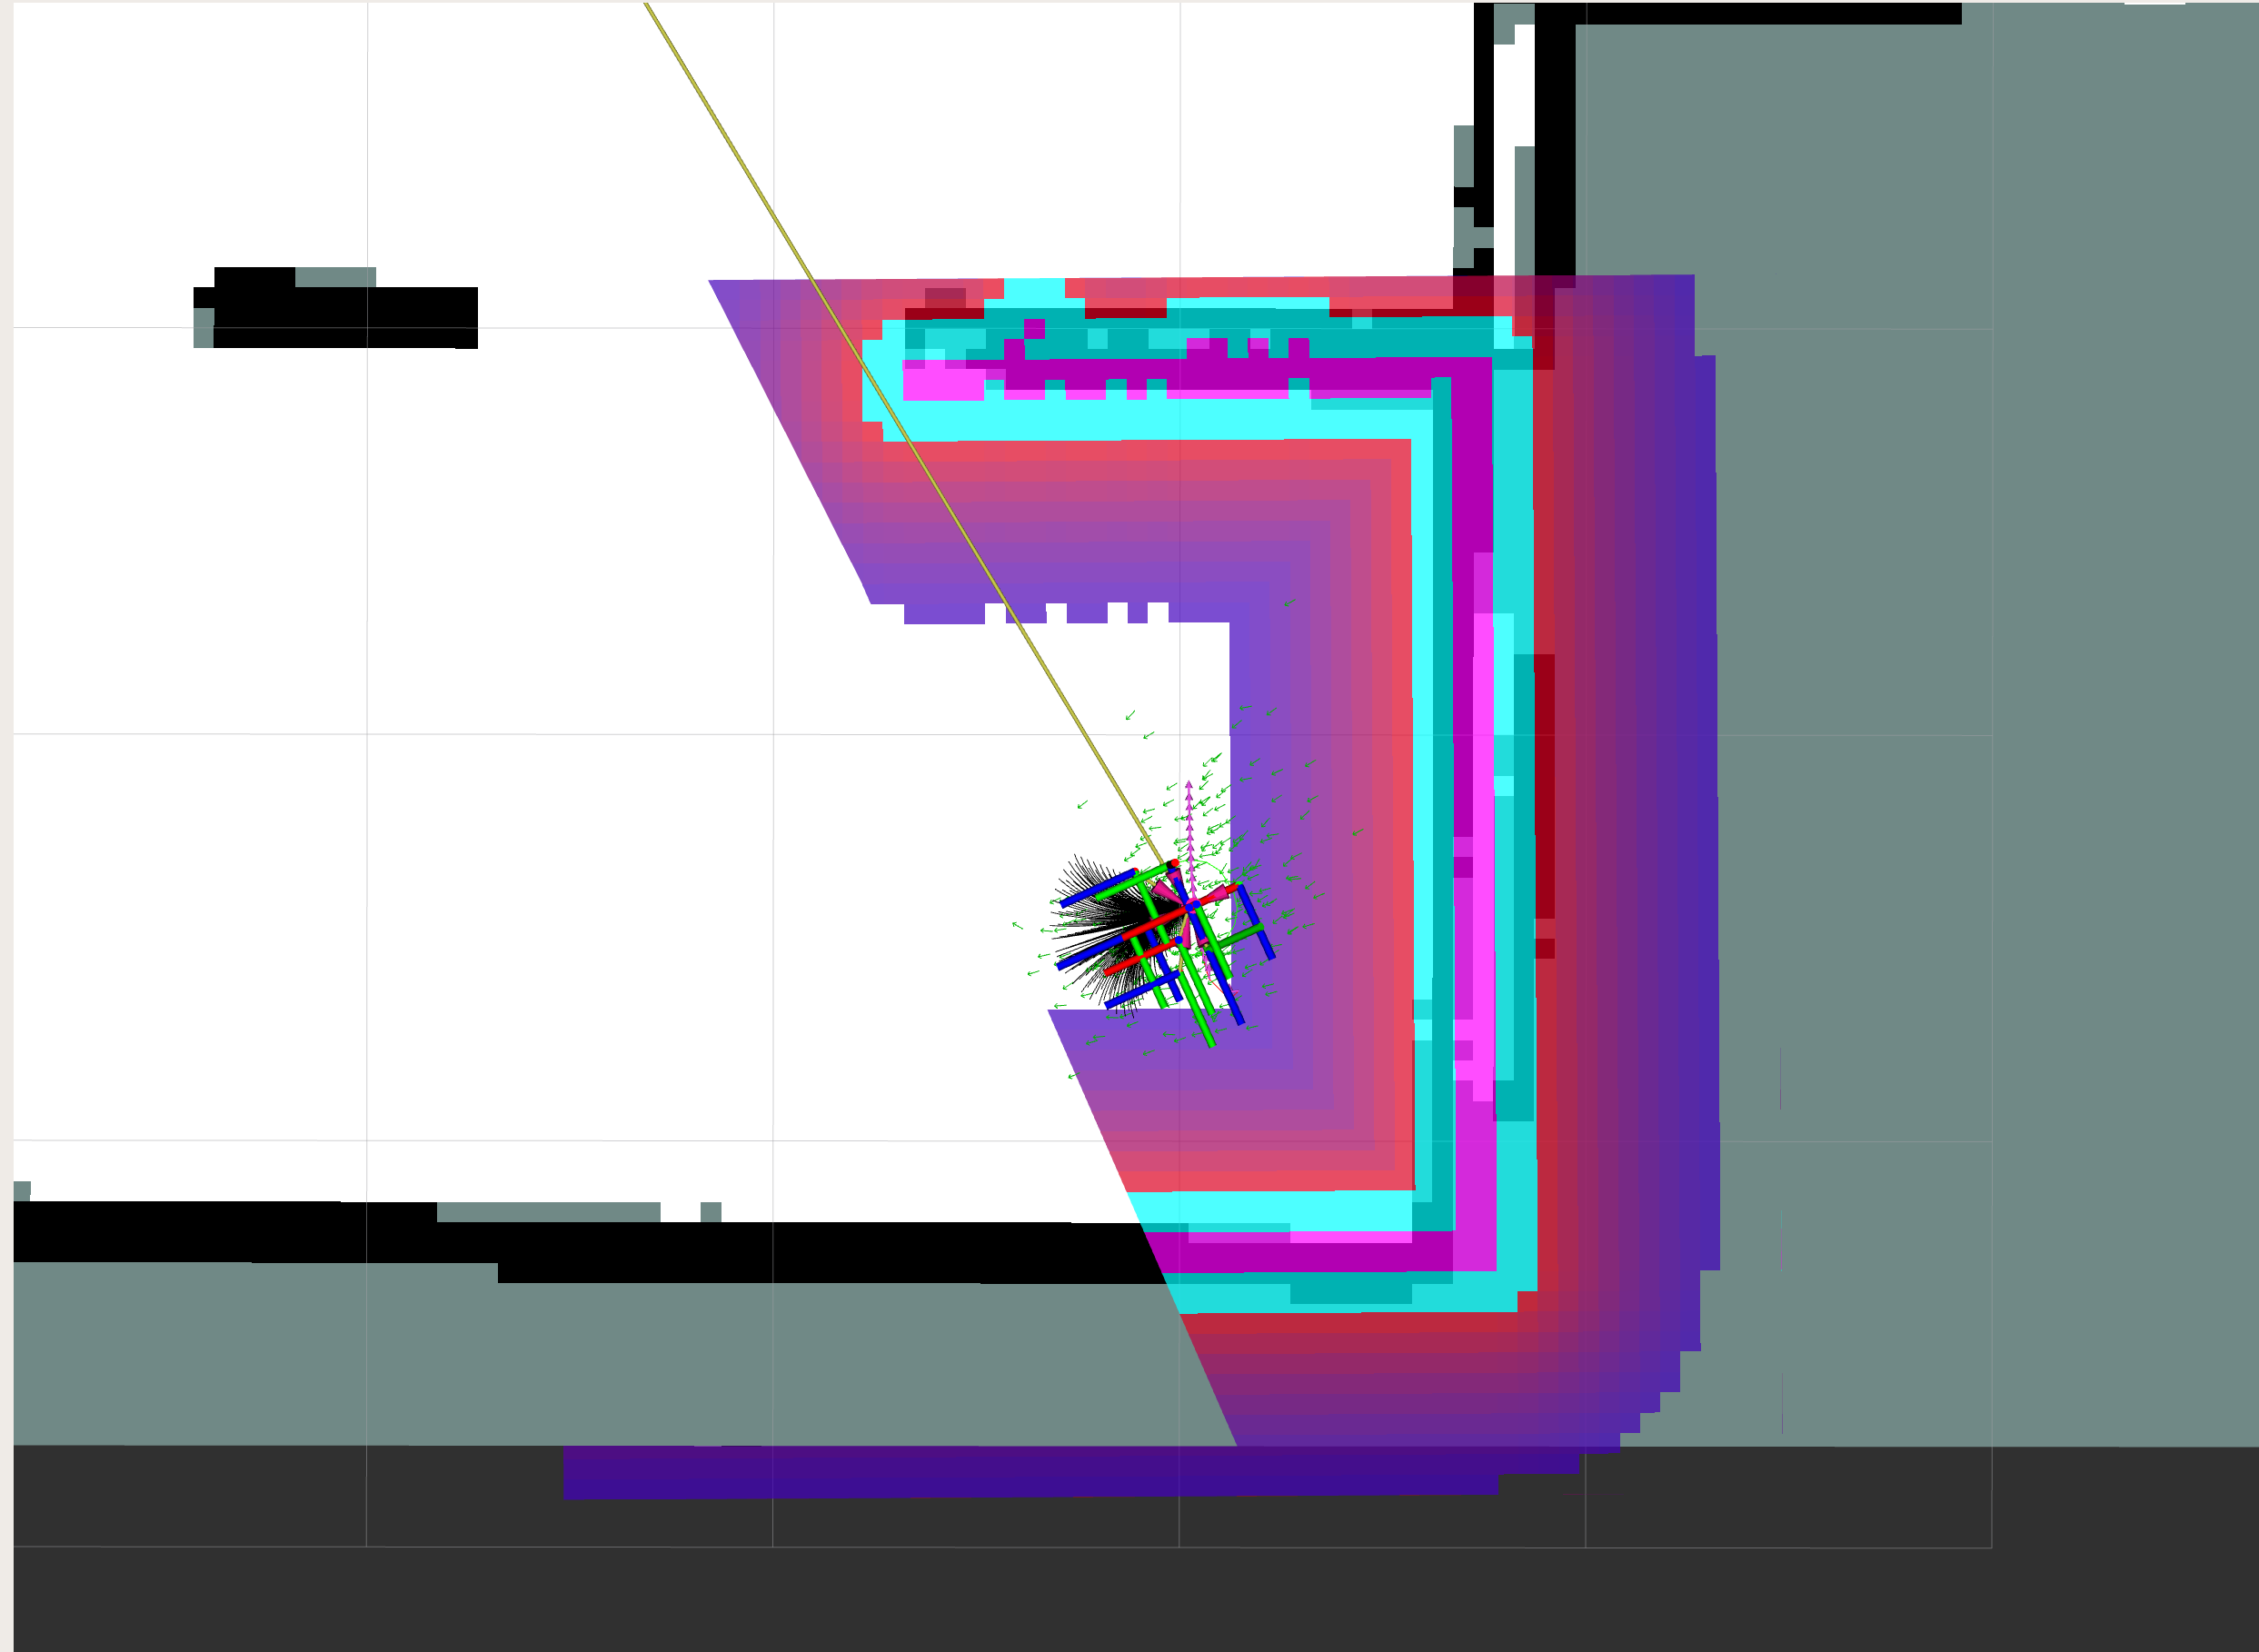
\includegraphics[width=\linewidth]{navigation_detail.png}
  \caption{Detailed navigation result} 
  \label{fig:navigation_detail}
\end{figure}{}
%%%%%%%%%%%%%%%%%%%%%%%%%%%%%%%%%%%%%%%%%%%%%%%%%%%%%%%%%%%%%%%%%%%%%%%%%%%%%%%%
\section{Conclusions}\label{conclusions}
ROS 2 is a amazing tool for Robotics application development. However, ROS 2 is still under heavy development, packages are constantly being updated, therefore it might still be too early to fully adapt ROS 2. 


ROS2 has many new features that are very convenient, such as the new launch system, this allows user to set environment variables easily through launch file rather than manually type into the comment line. 
%%%%%%%%%%%%%%%%%%%%%%%%%%%%%%%%%%%%%%%%%%%%%%%%%%%%%%%%%%%%%%%%%%%%%%%%%%%%%%%%
% \section{Reference}\label{reference}
\addtolength{\textheight}{-12cm}   % This command serves to balance the column lengths
                                  % on the last page of the document manually. It shortens
                                  % the textheight of the last page by a suitable amount.
                                  % This command does not take effect until the next page
                                  % so it should come on the page before the last. Make
                                  % sure that you do not shorten the textheight too much.
%%%%%%%%%%%%%%%%%%%%%%%%%%%%%%%%%%%%%%%%%%%%%%%%%%%%%%%%%%%%%%%%%%%%%%%%%%%%%%%%
\section*{APPENDIX}

%%%%%%%%%%%%%%%%%%%%%%%%%%%%%%%%%%%%%%%%%%%%%%%%%%%%%%%%%%%%%%%%%%%%%%%%%%%%%%%%
\section*{ACKNOWLEDGMENT}
%%%%%%%%%%%%%%%%%%%%%%%%%%%%%%%%%%%%%%%%%%%%%%%%%%%%%%%%%%%%%%%%%%%%%%%%%%%%%%%%
\begin{thebibliography}{99}

\bibitem{c1} Y. Maruyama, S. Kato, and T. Azumi, “Exploring the performance of ROS2,” Proceedings of the 13th International Conference on Embedded Software - EMSOFT 16, 2016. 
\bibitem{c2} Open Source Robotics Foundation(OSRF) http://www.osrfoundation.org/.
\bibitem{c3} Gerkey, B. (2019). Why ROS 2?. [online] Design.ros2.org. Available at: https://design.ros2.org/articles/why\_ros2.html [Accessed 9 Jul. 2019].
\bibitem{c6}Ros.org. (2019). Morgan Quigley (OSRF): ROS 2 on "Small" Embedded Systems - ROS robotics news. [online] Available at: http://www.ros.org/news/2016/03/morgan-quigley-osrf-ros-2-on-small-embedded-systems.html [Accessed 15 Jul. 2019].
\bibitem{c4} GitHub. (2019). ros2/ros1\_bridge. [online] Available at: https://github.com/ros2/ros1\_bridge [Accessed 9 Jul. 2019].
\bibitem{c5} ROBOTIS. (2019). ROBOTIS. [online] Available at: http://en.robotis.com/ [Accessed 15 Jul. 2019].
\bibitem{c7} "Using colcon to build packages", Index.ros.org, 2019. [Online]. Available: https://index.ros.org/doc/ros2/Tutorials/Colcon-Tutorial/. [Accessed: 16- Jul- 2019].
\end{thebibliography}
\end{document}
